\documentclass[aspectratio=169, 14pt]{beamer}
\usepackage[utf8]{inputenc}
\usepackage[english]{babel}
\usepackage{tipa}
\usepackage{graphicx}
\usepackage{transparent}
\usepackage{xeCJK}
\usepackage[ruled, lined, linesnumbered, commentsnumbered]{algorithm2e}
\usepackage{tikz}
\usetikzlibrary{calc,shadows.blur}
\usetikzlibrary{matrix,backgrounds}
\usepackage{pgfplots}
\pgfplotsset{compat=1.13}
\usepackage{minted}
\usepackage{csquotes}
\usepackage{outlines}
\usepackage{booktabs}
\usepackage{fontawesome5}
\usepackage{hyperref}
\hypersetup{
	colorlinks=true,
	linkcolor=blue,
	filecolor=magenta,
	urlcolor=cyan,
}
\urlstyle{same}
\usetheme{metropolis}
\metroset{block=fill}
\usecolortheme{default}
\definecolor{darkmidnightblue}{rgb}{0.0, 0.2, 0.4}
\definecolor{LightGray}{gray}{0.9}


%------------------------------------------------------------
%This block of code defines the information to appear in the
%Title page
\title[Data Structures] %optional
{Data Structures}

\subtitle{Algorithm Analysis}

\author[CHEN Zhongpu] % (optional)
{CHEN Zhongpu}

\institute[] % (optional)
{
	School of Computing and Artificial Intelligence \\
	\href{mailto:zpchen@swufe.edu.cn}{zpchen@swufe.edu.cn}
}

\date[] % (optional)
{SWUFE, Fall \the\year{}}

%End of title page configuration block
%------------------------------------------------------------


%------------------------------------------------------------
%The next block of commands puts the table of contents at the 
%beginning of each section and highlights the current section:

% \AtBeginSection[]
% {
%   \begin{frame}
%     \frametitle{Table of Contents}
%     \tableofcontents[currentsection]
%   \end{frame}
% }
%------------------------------------------------------------


\begin{document}

%The next statement creates the title page.
\frame{\titlepage}

%---------------------------------------------------------
%This block of code is for the table of contents after
%the title page
% \begin{frame}
% \frametitle{Table of Contents}
% \tableofcontents
% \end{frame}
%--------------------------------------------------------
\begin{frame}[fragile]
	\frametitle{A Small Quiz}
	\begin{enumerate}
		\item How to access the last element of a \alert{list} in Python?
		\item What does the following code snippet do?
	\end{enumerate}

	\begin{minted}[bgcolor=LightGray]{python}
a = [i for i range(10)]
b = [1] * 10
    \end{minted}
\end{frame}

{
% \usebackgroundtemplate{\transparent{0.3}{\begin{picture}
%     \includegraphics[height=0.7\paperheight]{cover}
% \end{picture}    
% }}
\usebackgroundtemplate{
	\tikz[overlay,remember picture]
	\node[opacity=0.3, at=(current page.south east),anchor=south east, yshift=2cm,xshift=4cm] {
		\includegraphics[height=0.6\paperheight]{cover}};
}
\begin{frame}
	\section{\textcolor{darkmidnightblue}{1. Algorithm Analysis}}
\end{frame}
}

\begin{frame}[fragile]
	\frametitle{1.1 How Fast Is A Program?}
	\begin{block}{Fact 2}
		\textbf{Different data structures have varying (time) \alert{efficiencies}.}
	\end{block}
	A straightforward way is to measure the elapsing time.
	\begin{minted}[bgcolor=LightGray, fontsize=\small]{python}
import time
start = time.time()
# your program runs
end = time.time()
elapse = end - start
\end{minted}
	A more robust way is to use \alert{timeit} module.
\end{frame}

\begin{frame}[fragile]
	\texttt{1, 1, 2, 3, 5, 8, 13, ...}
	\begin{minted}[bgcolor=LightGray, fontsize=\small]{python}
def fibonacci(n):
    if n == 0:
        return 0
    elif n == 1 or n == 2:
        return 1
    else:
        return fibonacci(n - 1) + fibonacci(n - 2)        
    \end{minted}
	Which will cost more time? \texttt{fibonacci(10)}, or \texttt{fibonacci(20)}?

	Intuitively, the time cost grows with the \textbf{input size} (\emph{problem size}).
\end{frame}


\begin{frame}[fragile]
	Still, you will find yourself asking the more detailed question: \textbf{How long will my program take, as a function of the input size?}

	\begin{minted}[bgcolor=LightGray, fontsize=\small]{python}
if __name__ == '__main__':
    ns = [i for i in range(20, 31)]
    with open('fib_python.txt', 'w') as f:
        for n in ns:
            start = round(time.time() * 1000)
            fibonacci(n)
            end = round(time.time() * 1000)
            f.write(f'{n}   {end - start}\n')
\end{minted}

\end{frame}

\begin{frame}
	\frametitle{Plot}
	\begin{columns}
		\column{0.5\textwidth}
		\begin{center}
			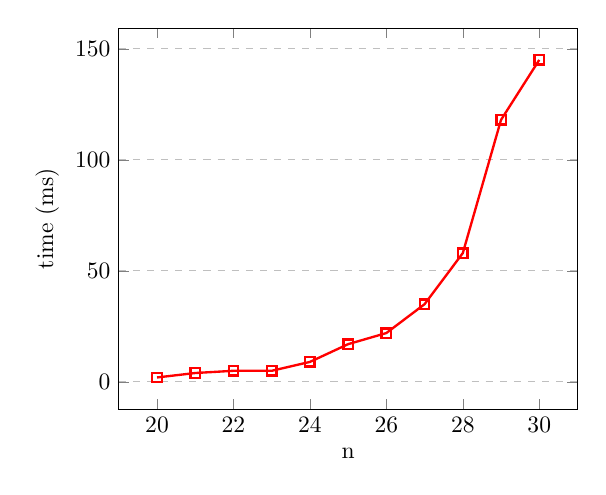
\begin{tikzpicture}[scale=0.85]
				\begin{axis}[
						xlabel={n},
						ylabel={time (ms)},
						ymajorgrids=true,
						grid style=dashed,
					]

					\addplot[
						color=red,
						mark=square,
						line width=1pt,
					]
					coordinates {
							(20, 2)(21, 4)(22, 5)(23, 5)(24, 9)(25, 17)(26, 22)(27, 35)(28,58)(29,118)(30,145)
						};

				\end{axis}
			\end{tikzpicture}
		\end{center}
		\column{0.45\textwidth}
		Popular visualization tools:  \texttt{gnuplot}, \texttt{ggplot2} in R, \texttt{Matplotlib} in Python, and \texttt{Plotly Express} in Python.

	\end{columns}
\end{frame}

\begin{frame}[fragile]
	\frametitle{Mathematical Models}
	\begin{block}{Motivation}
		To analyze an algorithm, a \alert{mathematical model} is needed in addition to the empirical experiments due to the following reasons:
	\end{block}
	\begin{enumerate}
		\item<1-> To compare different algorithms is feasible unless the hardware and software environments are the same.
		\item<2-> Experiments can be done only a limited set of test inputs.
		\item<3-> An algorithm must be fully implemented before the experiments.
	\end{enumerate}
\end{frame}

\begin{frame}

	\begin{exampleblock}{Knuth's insight}
		The total running time of a program is determined by two primary factors:
		\begin{enumerate}
			\item The cost of executing each statement
			\item The frequency of execution of each statement
		\end{enumerate}
	\end{exampleblock}

	We assume that \alert{primitive operations} take \alert{constant} time to execute.

	Therefore, \textbf{the running time of a program is proportional to the number of primitive operations executed.}

\end{frame}

\begin{frame}[fragile]

	{\large \faIcon{question-circle}} What is the cost of the following function?
	\begin{minted}[bgcolor=LightGray,]{python}
def foo(n):
    for i in range(n):
        print(i)
\end{minted}

	{\large \faIcon{question-circle}} What is the cost of the following function?
	\begin{minted}[bgcolor=LightGray]{python}
def cubic_sum(n):
    s = 0
    for i in range(1, n+1):
        s += i * i * i
    return s
\end{minted}
\end{frame}

\begin{frame}[fragile]

	{\large \faIcon{question-circle}} What is the frequency of the inner \alert{if} statement?
	\begin{minted}[bgcolor=LightGray]{python}
    def two_sum(self, nums, target):
        for i, v in enumerate(nums):
            for j in range(i + 1, len(nums)):
                if v + nums[j] == target:
                    return [i, j]
        return []
    \end{minted}


\end{frame}

\begin{frame}[fragile]
	\begin{block}{Revisit}
		Suppose there are $10^6$ books in an array. To find a book titled \emph{"Gone with the wind"}, how many times is the comparison performed?
		\begin{enumerate}
			\item On the \textbf{best} case: 1
			\item On the \textbf{worst} case: $10^6$
			\item On the \textbf{average} case $10^6/2$
		\end{enumerate}
	\end{block}

	\begin{tikzpicture}
		\node[fill=yellow,blur shadow={shadow xshift=-0.5ex},
			text width=24em,anchor=south west,rounded corners]
		{\faIcon{lightbulb} We only focus on the \alert{worst-case running time} in this course.};
	\end{tikzpicture}

\end{frame}

\begin{frame}[fragile]
	\frametitle{Order of Growth}
	We can simplify the cost model by taking a "big-picture" approach: it is the \alert{order of growth} (rate of growth) of the running time as a function of the input size.

	\begin{table}
		\begin{tabular}{lll}
			\toprule
			Function              & Approximation & Order of growth \\
			\midrule
			$n^3/6 - n^2/2 + n/3$ & $n^3/6$       & $n^3$           \\
			$n^2/2 - n/2$         & $n^2/2$       & $n^2$           \\
			$\lg{n} + 1$          & $lg{n}$       & $lg{n}$         \\
			$3$                   & $3$           & $1$             \\
			\bottomrule
		\end{tabular}
	\end{table}
\end{frame}
\begin{frame}[fragile]

	\begin{columns}
		\column{0.4\textwidth}
		Compare $\frac{n^2 - n}{2}$ and $\frac{n^2}{2}$.

		We can say \alert{$\frac{n^2}{2} \sim \frac{n^2 - n}{2}$}, because $\frac{n^2}{2}$ is similar to $\frac{n^2 - n}{2}$ as $n$ grows. And the \textbf{order of growth} is $n^2$.

		\column{0.6\textwidth}
		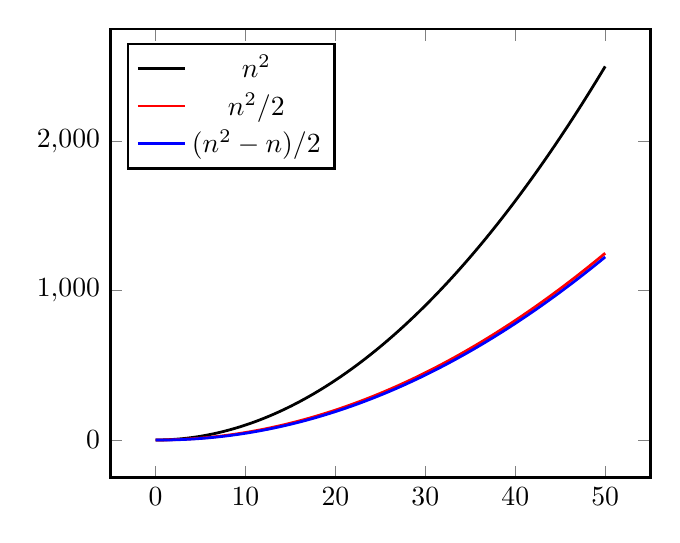
\begin{tikzpicture}
			\begin{axis}[legend pos=north west,line width=1pt]
				\addplot[domain=0:50,samples=100]{x*x};
				\addlegendentry{\(n^2\)}
				\addplot[color=red, domain=0:50,samples=100]{x*x/2};
				\addlegendentry{\(n^2/2\)}
				\addplot[color=blue, domain=0:50,samples=100]{(x*x - x)/2};
				\addlegendentry{\((n^2-n)/2\)}
			\end{axis}
		\end{tikzpicture}
	\end{columns}
\end{frame}


\begin{frame}[fragile]

	\begin{center}
		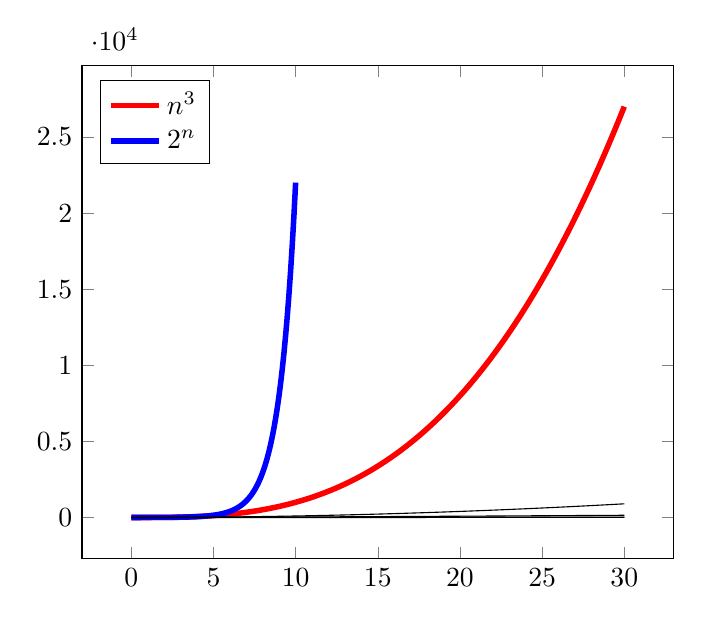
\begin{tikzpicture}
			\begin{axis}[legend pos=north west, width=.75\textwidth]
				\addplot[color=red, domain=0:30,samples=100, line width=2pt]{x^3};
				\addlegendentry{\(n^3\)}
				\addplot[color=blue, domain=0:10, samples=100, line width=2pt]{exp(x)};
				\addlegendentry{\(2^n\)}
				\addplot[domain=0:30,samples=100]{1};
				\addplot[domain=0:30,samples=100]{log2(x)};
				\addplot[domain=0:30,samples=100]{x};
				\addplot[domain=0:30,samples=100]{x*log2(x)};
				\addplot[domain=0:30,samples=100]{x^2};
			\end{axis}
		\end{tikzpicture}
	\end{center}

\end{frame}

\begin{frame}[fragile]
	\begin{center}
		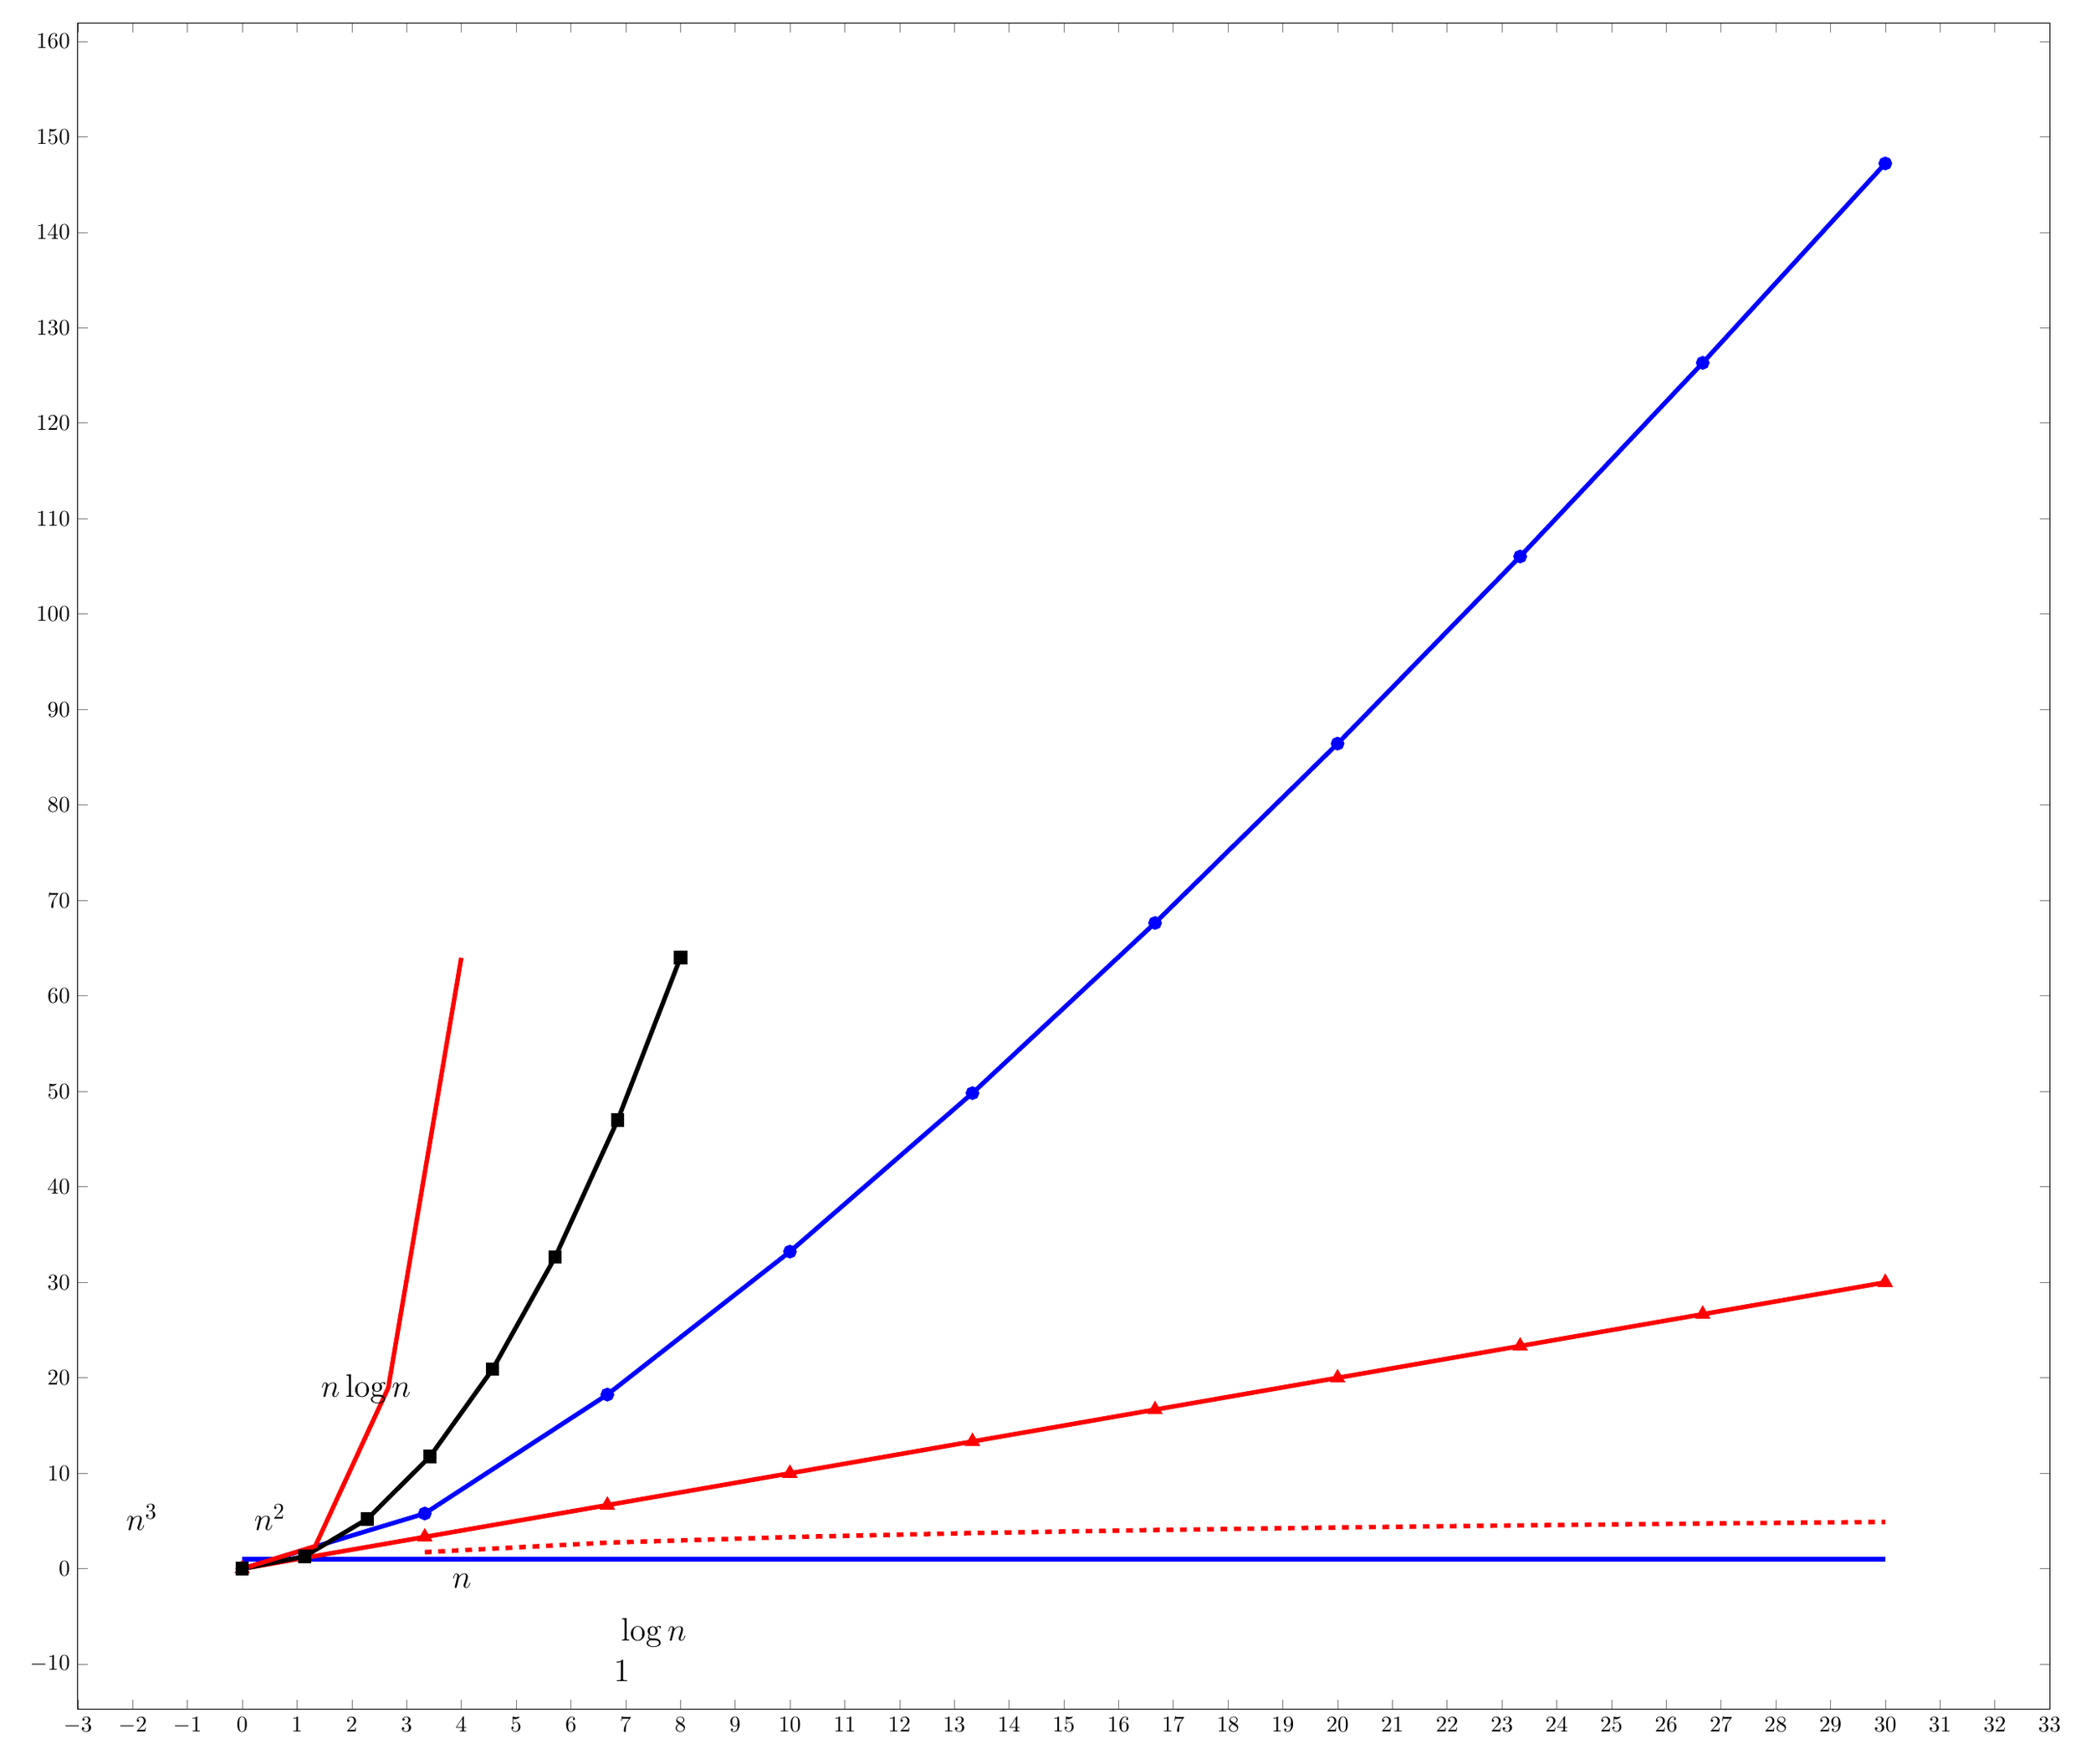
\begin{tikzpicture}
			\begin{axis}[legend pos=north west, height=1\paperheight]
				\addplot[blue, domain=0:30,samples=100, line width=2pt]{1};
				\addplot[domain=0:30,samples=10, dashed, red, line width=2pt]{log2(x)};
				\addplot[red, mark=triangle*, domain=0:30,samples=10, line width=2pt]{x};
				\addplot[blue, mark=*,domain=0:30,samples=10, line width=2pt]{x*log2(x)};
				\addplot[mark=square*, domain=0:8,samples=8, line width=2pt]{x^2};
				\addplot[red, domain=0:4, samples=4, line width=2pt]{x^3};
			\end{axis}
			\node at (1, 3) {\Large $n^3$};
			\node at (3, 3) {\Large $n^2$};
			\node at (4.5, 5) {\Large $n\log{n}$};
			\node at (6, 2) {\Large $n$};
			\node at (9, 1.2) {\Large $\log{n}$};
			\node at (8.5, 0.6) {\Large $1$};
		\end{tikzpicture}
	\end{center}


\end{frame}
\begin{frame}
	\frametitle{1.2 Big O Notation}

	\begin{columns}
		\column{0.4\textwidth}
		The order of growth is often described by the \alert{big O} notation.

		\column{0.59\textwidth}
		\begin{table}
			% \caption{Common time complexity descriptions}
			\begin{tabular}{ll}
				\toprule
				Description  & Time complexity \\
				\midrule
				constant     & $O(1)$          \\
				logarithmic  & $O(log{n})$     \\
				linear       & $O(n)$          \\
				linearithmic & $O(nlog{n})$    \\
				quadratic    & $O(n^2)$        \\
				cubic        & $O(n^3)$        \\
				exponential  & $O(2^n)$        \\
				\bottomrule
			\end{tabular}
		\end{table}
	\end{columns}
\end{frame}

\begin{frame}

	\begin{exampleblock}{Big O}
		Suppose $f(x)$ and $g(x)$ are two functions defined on some subset of the real numbers. We write
		\[f(x) = O(g(x))\]
		if and only if there exists constants $N$ and $C$ such that
		\[f(x) \leq Cg(x), \forall x > N\]
	\end{exampleblock}

	Intuitively, this means that $f$ does not grow faster than $g$ ($g$ is the \alert{upper bound} of $f$).

\end{frame}

\begin{frame}
	Big-O denotes the \textbf{"less-than-or-equal-to"} concept:

	\[7n^3 + 100n^2 - 20n + 6\]

	We can say the order of growth is $n^3$. To put it in another way, this function grows no faster than $n^3$, so we can write that it is $O(n^3)$.
\end{frame}

\begin{frame}[fragile]
	\frametitle{Example}
	\begin{enumerate}
		\item The function $8n + 5$ is $O(n)$.
		\item The function $n^2 + 2n + 1$ is $O(n^2)$.
		\item The function $5n^2 + 3n\log{n} + 2n + 5$ is $O(n^2)$.
		\item The function $3\log{n} + 2$ is $O(\log{n})$.
		\item The function $8n + 5$ is $O(8n + 5)$.
		\item The function $8n + 5$ is $O(n^2)$.
	\end{enumerate}
	\pause

	\begin{tikzpicture}
		\node[fill=yellow,blur shadow={shadow xshift=-0.5ex},
			text width=26em,anchor=south west,rounded corners]
		{\faIcon{lightbulb} We should use big-O in \alert{tightest and simplest} terms.};
	\end{tikzpicture}
\end{frame}

\begin{frame}[fragile]

	{\large \faIcon{question-circle}} What is the time complexity in 	\begin{minted}[bgcolor=LightGray]{python}
def foo(n):
    for i in range(n):
        print(i)
    \end{minted}

	\begin{minted}[bgcolor=LightGray, baselinestretch=1]{python}
def two_sum(self, nums, target):
    for i, v in enumerate(nums):
        for j in range(i + 1, len(nums)):
            if v + nums[j] == target:
                return [i, j]
    return []
    \end{minted}
\end{frame}

\begin{frame}[fragile]
	\begin{minted}[bgcolor=LightGray]{python}
def search(a, target):
    for i, v in enumerate(a):
        if v == target:
            return i
    return -1
\end{minted}
\end{frame}

\begin{frame}[fragile]
	\begin{minted}[bgcolor=LightGray]{python}
def search(a, target):
    high = len(a) - 1
    low = 0
    while high >= low:
        mid = low + (high - low) // 2
        if a[mid] == target:
            return mid
        elif a[mid] > target:
            high = mid - 1
        else:
            low = mid + 1
    return -1
\end{minted}

\end{frame}

\begin{frame}
	\frametitle{Some Words of Caution}
	Do the following statements make sense?

	\begin{itemize}
		\item Since $n^2 - n = O(n^2)$ and $n^2 - 1 = O(n^2)$, we can say $n^2 - n = n^2 - 1$.
		\item An algorithm in $O(n)$ is always faster than an algorithm in $O(n^3)$.
	\end{itemize}

\end{frame}

\begin{frame}
	\frametitle{1.3 Revisit Fibonacci}
	\begin{columns}
		\column{0.6\textwidth}
		\begin{center}
			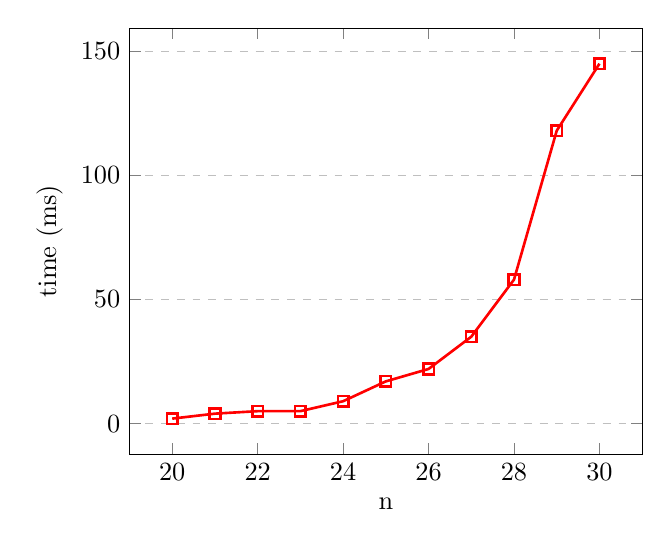
\begin{tikzpicture}[scale=0.95]
				\begin{axis}[
						xlabel={n},
						ylabel={time (ms)},
						ymajorgrids=true,
						grid style=dashed,
					]

					\addplot[
						color=red,
						mark=square,
						line width=1pt,
					]
					coordinates {
							(20, 2)(21, 4)(22, 5)(23, 5)(24, 9)(25, 17)(26, 22)(27, 35)(28,58)(29,118)(30,145)
						};

				\end{axis}
			\end{tikzpicture}
		\end{center}
		\column{0.4\textwidth}
		The time complexity of fibonacci is $O(2^n)$.

	\end{columns}

\end{frame}

\begin{frame}
	\frametitle{1.4 A Final Note}
	\begin{alertblock}{Note}
		A comprehensive about algorithm analysis is out of the scope of this course.
	\end{alertblock}

	\begin{itemize}
		\item $\Theta(n)$
		\item $\Omega(n)$
	\end{itemize}
\end{frame}


\begin{frame}
	\section{\textcolor{darkmidnightblue}{Conclusion}}

	\begin{enumerate}
		\item Big O notation
		\item Evaluation through visualization
	\end{enumerate}
\end{frame}

{
\usebackgroundtemplate{
	\tikz[overlay,remember picture]
	\node[opacity=0.3, at=(current page.south east),anchor=south east, yshift=2cm,xshift=4cm] {
		\includegraphics[height=0.6\paperheight]{cover}};
}
\begin{frame}
	\section{\textcolor{darkmidnightblue}{Design an Array}}
\end{frame}
}

\begin{frame}
	\frametitle{Some Facts}
	\begin{exampleblock}{Array}
		An array is a container object that holds a fixed number of values of a single type.
	\end{exampleblock}
	\begin{enumerate}
		\item A list in Python is NOT an array.
		\item Python has module \href{https://docs.python.org/3/library/array.html}{array}, but it is mainly used for the sake of performance.
	\end{enumerate}
\end{frame}

\begin{frame}[fragile]
	\frametitle{Design Goal}
	To implement an array-like fixed-size data structure, we need to support the following operations:

	\begin{minted}[bgcolor=LightGray]{python}
arr = Array(5)
print(len(arr))
arr[4] = 7
print(arr[4])
for i in arr:
  print(i)
\end{minted}
\end{frame}

\begin{frame}[fragile]
	\frametitle{How to save data}
	We use the list as the underlying (private) data structure:
	\begin{minted}[bgcolor=LightGray]{python}
class Array:
    def __init__(self, n):
        self._data = [0] * n
        self._size = n
\end{minted}
\end{frame}

\begin{frame}[fragile]
	\frametitle{How to get the length}
	The traditional way:

	\begin{minted}[bgcolor=LightGray]{python}
class Array:
    def get_size(self):
        __________
\end{minted}
	A more \alert{Pythonic} way (using \textbf{special methods}):
	\begin{minted}[bgcolor=LightGray]{python}
class Array:
    def __len__(self):
        __________
\end{minted}
\end{frame}

\begin{frame}[fragile]
	\frametitle{How to set and get elements}
	\begin{minted}[bgcolor=LightGray]{python}
    def __getitem__(self, i):
        return self._data[i]

    def __setitem__(self, value, i):
        self._data[i] = value
\end{minted}
	\pause
	\begin{tikzpicture}
		\node[fill=yellow,blur shadow={shadow xshift=-0.5ex},
			text width=26em,anchor=south west,rounded corners]
		{\faIcon{lightbulb} A class with \alert{\_\_len\_\_()} and \alert{\_\_getitem\_\_()} is \alert{iterable}.};
	\end{tikzpicture}
\end{frame}

\begin{frame}[fragile]
	\frametitle{Exercise}
	Try to update init method which accepts a list of values, instead of its size.
	\begin{minted}[bgcolor=LightGray]{python}
arr = Array(1, 2, 3, 4, 5)
\end{minted}
	Also, try to use it as a vector, and add methods for vector-addition and vector-subtraction.
	\begin{minted}[bgcolor=LightGray, fontsize=\small]{python}
a = Array(1, 2, 3, 4, 5)
b = Array(5, 4, 3, 2, 1)
# a + b = Array(6, 6, 6, 6, 6)
# a - b = Array(-4, -2, 0, 2, 4)
\end{minted}
\end{frame}

\end{document}
